\documentclass{standalone}
\usepackage{tikz}

\begin{document}
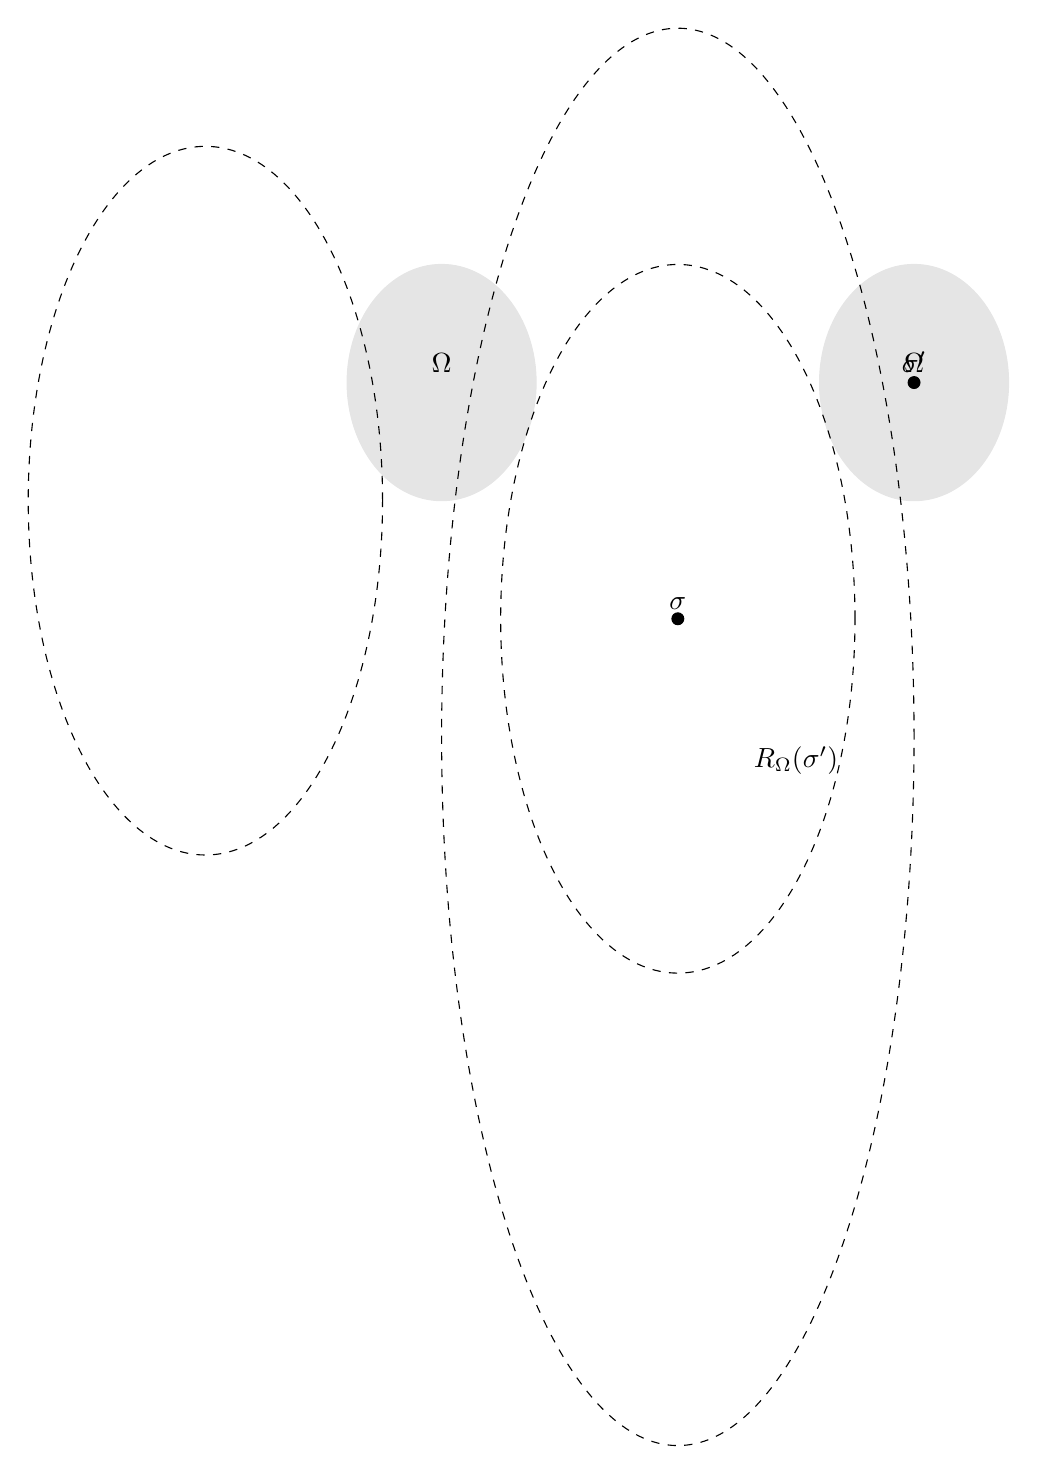
\begin{tikzpicture}[scale=1.5]
    \filldraw[gray!20] (0,0) ellipse (0.8 and 1);
    
    % Define the circle for RΩ(σ)
    \path[draw,dashed] (-2,-1) circle [x radius=1.5cm,y radius=3cm];
    
    \filldraw[gray!20] (4,0) ellipse (0.8 and 1);
    \filldraw[black] (4,0) circle (0.05);
    \node at (4,0) [above] {$\sigma'$};
    
    % Define the circle for RΩ(σ')
    \path[draw,dashed] (2,-3) circle [x radius=2cm,y radius=6cm];
    
    \filldraw[white] (3.7,-3) rectangle ++(-1,0.5);
    \node at (3,-3) [below] {$R_\Omega(\sigma')$};
    
    % Label for Ω
    \node at (0,0) [above] {$\Omega$};
    \node at (4,0) [above] {$\Omega$};
    
    % Define the circle for σ
    \path[draw,dashed] (2,-2) circle [x radius=1.5cm,y radius=3cm];
    
    \filldraw[black] (2,-2) circle (0.05);
    \node at (2,-2) [above] {$\sigma$};
\end{tikzpicture}
\end{document}